\chapter{Methods, techniques, tools}\label{chapter:methods}
%\section{Introduction}\label{methods:intro}
This chapter introduces the representation of agents and obstacles within the swarm environment and the algorithms applied to inter-agent and obstacle interactions to produce a swarming effect. Movement of agents and the application of the directional bias for goal based swarms are presented mathematically for modelling ~\cite{MP:10}. 

Currently most research uses field effects as the method of modelling inter-agent interactions~\cite{BAF:06, BAFVM:06, BM:09, APZDAMC:09, GP:02, GP:04, GP:04a, GP:05, GP:11, MYP:09}. The models usually use two field effects to implement the swarming characteristic. These effects are cohesion, to draw agents closer, and repulsion to prevent agents colliding. Field effects are the ranges around an agent that determine the effect other agents have upon its movement. When an agent moves into the outermost field effect, which is usually the cohesion field effect, of another agent it is considered to be a neighbour. A common approach to the application of the field effects is to use fixed ranges common to all agents. Cohesion is applied based on neighbour proximity and repulsion is applied at a fixed level when an agent is within the repulsion field. This chapter uses a similar cohesion effect and introduces a graduated field effect based on neighbour agent proximity for repulsion when calculating an agent's movements.

\section{Modelling agents}
Modelling a swarm requires a representation of agents, their movements, and their interactions. Swarm agents are modelled as a point in 2 dimensional space with no mass or size. This representation is used by Vankerkom and Yu when visualising swarms~\cite{VY:04}. Mohan and Ponnambalam, and Gazi and Passino~\cite{VY:04, GP:04} use the same representation and also model agents moving at a constant speed. These concepts are used in most research that involves multi-agent interactions such as the work by Barnes et al. and Bennet~\cite{BAF:06, BAFVM:06, BFV:07, BM:09} and Andreou et al.~\cite{APZDAMC:09}.

The model is built using vectorial and geometric techniques~\cite{HER:11, BAF:06}. The position of agents is modelled using cartesian coordinates and the movements are modelled using vectors. The coordinates of an agent are the component of the position vector; a movement is the addition of a vector to this position vector.

%% The mathematical tecniques used to achieve the modelling are geometry and vector mathematics~\cite{HER:11, BAF:06}. The positional aspects of agents are modelled in the form of coordinate geometry and the movements are modelled using vector mathematics. These modelling techniques are highlighted in surveys carried out by Holmstr{\"o} and Romero~\cite{HR:ND}, Minor~\cite{MIN:07} and Muniganti and Pujol~\cite{MP:10}. 

Swarms can be modelled in two~\cite{MIN:07, VY:04} or three~\cite{BSB:15} dimensions.
This thesis uses a two dimentional model with unbounded ranges.
%% \section{Swarming plane}
%% The modelling of swarms can be carried out in two dimensional planes. Swarms can be modelled in three dimensional space using the three axis of $x,y,z$~\cite{BSB:15} or two dimensional space using $x,y$~\cite{MIN:07, VY:04}.
%%  
%% This thesis uses a 2D Euclidean plane $(x,y)$. The dimensions of the plane are unlimited $(-\infty< x,y <+\infty)$ with a central origin of $(0,0)$. All the techniques discussed in this thesis could be transitioned to 3D space~\cite{PG:08} as a 2D environment can be considered as being a 3D environment with the $z$ axis set to $0$. 
                                
%% \section{Environment modelling principle}\label{method:RealNumberModelling}
%% Each agent's position within a swarm is modelled as a point consisting of two floating point numbers to represent their $(x,y)$ position.

\section{Modelling agent and environment interactions}\label{method:AgentEnvironmentModel}
For the agents within a swarm to be modelled  the environemnet must allow additional objects that the agents will interact with.
Positions of objects are computed relative to an agent of interest. Objects of interest are other agents, obstacles and destinations. Obstacles can be considered as a point in space with an associated repulsion field effect and a destination is a point within the Euclidian plane that agents migrate towards.
%% Modelling of the swarm will be performed using two techniques; vectors for inter-object interactions and coordinates for positional locations. The proximity of each of the objects within the swarm are identified, the objects being, agents, obstacles and destinations. The effects of the objects upon each other are determined using fixed ranges (field effects). 
This modelling technique is similar to that used by Barnes et al.~\cite{BAF:06, BAFVM:06}. The distribution of each of these objects, along with the field effects, produce sets of vectors that represent the inter-object influences in the system. The vector sets for each agent are used to calculate an interim directional vector for each interaction type (cohesion, repulsion, direction), this is similar to the techniques used by Jung et al. and Saldaña et al.~\cite{JG:13, SOM:12}. Altering the influence of these vector sets using a weighting produces a directional vector~(\autoref{methods:weightedModel}). This resultant vector is normalised to produce a directional vector that can be used to create movement~\cite{KC:08}. The agent's speed characteristic is used along with the discrete time cycle ($t$)~\cite{FAP:05, GP:05} to determine an agent's next position.

\section{Modelling time}
There are two options for representing time when modelling a swarm: continuous time and discrete time. Continuous time~\cite{HW:08} is where between two points in time there is another point. Discrete time~\cite{FAP:05, GP:05, RVMH:13, HER:11, MP:10, PCL:08a} is where there are identifiable points of time between two events. In this thesis discrete time is used. This approach has been used in many projects as identified by Muniganti and Pujol in their survey of mathematical swarming models~\cite{MP:10}. 

\section{Swarming algorithms} 
The logic that produces the cooperative appearance of agents in a swarm are the algorithms that each agent applies to calculating their movement~\cite{BS:13, DLK:11, HAY:08}. There are many variation in how algorithms apply their effects~\cite{BBBV:04, DT:03}. The basis of all algorithms is that they consider two influencing factors, direction and speed~\cite{BAF:06, BAFVM:06, BVD:14, EP:10}. 

The application of the movement is therefore calculated using the time, speed and direction in discrete intervals as shown in~\autoref{method:SwarmParticipant} where $s_b$ is the agent speed, $t$ is time, $b$ is the agent and $v$ is the resultant vector that is used to calculate the movement.

\begin{figure}[H]
\begin{center}
\includegraphics[width=7cm]{CHAPTER-2/figures/SwarmParticipant}
\caption{Algorithm effects \label{method:SwarmParticipant}}
\end{center}
\end{figure}

%% \subsubsection{Swarming algorithms/model check} 
%% When calculating movement in a simulation the distance moved by the agents must be modelled in such a way that physically impossible scenarios do not occur. As agents are simulated mathematically it is possible for the simulation to calculate a path that would allow two agents to pass through the same space ($x,y$) at the same time. It is also possible to create environmental configurations that would allow an inter-object effect to be missed. This can be caused by the model not identifying agents passing through a field effect due to its calculated movement extending beyond or crossing a field effect in one time increment. 
%% These potential situations are eliminated by ensuring the sampling rate is a multiple of the clock cycle for calculating field effects, and the movement of an agent is less than any of the field effects. This check is incorporated into the simulator as a parameter check when the physics model of the graphical simulator is changed.

\section{Boid model modification}\label{methods:BoidModel}
Hereford~\cite{HER:11} and Barnes et al.~\cite{BAF:06} modelled static swarms using a bi-variable technique. The bi-variable components are cohesion and repulsion. 

Gazi and Passino also used this bi-variable technique to examine inter-agent interactions when creating stable swarm structures and ensuring agents remained part of a swarm while not colliding~\cite{GP:04a, GP:02, GP:04}. 

If a swarm is to be goal based then the swarm is modelled using three vector components, cohesion, repulsion, and a direction vector as discussed by Salda\~na et al., Stranders et al., Nash and Koenig~\cite{SOM:12, SRDF:10, NK:10}. 

The first swarming model to use three components was the Boid model. In the Boid model the directional component is determined by agents communicating locally to generate a consensus based direction. The consensus direction is then applied to create a `flocking' effect~\cite{KC:08, REY:87}. This cooperative method of deriving a directional bias can be seen in the formation of fish shoals~\cite{YGT:10, PMRT:14} and starling murmurations~\cite{CS:15, ZZLW:14, PMRT:14}. 

Barnes et al., Bennet and McInnes, Cai et al. Correl and Rus, Dinolov et al. and Ekanayake and Pathirana take a different approach to creating a directional bias~\cite{BAF:06, BAFVM:06, BM:09, CML:ND, CR:13, DLK:11, EP:10}. They generate a directional bias by creating a vector from an agent to a fixed destination, such as a simulated GPS position. This additional vector is then added to the cohesion and repulsion vectors which control the inter-agent interactions. Adding the directional bias creates a goal based characteristic.  

\section{Agent ranges}
All inter-agent interactions are determined by how close agents are to each other. When agents fall within a predetermined distance they are classed as neighbours. The set range for inclusion as a neighbour is referred to as the `neighbour range'~\cite{BAF:06, BAFVM:06}. In a physical implementation of a swarm the distance could be determined by some form of sensing device such as the omni-directional camera as used in the s-bot project~\cite{HR:ND}. 

\section{Swarm cohesion}\label{sec:Cohesion1}
Several views of cohesion exist within the swarm research community. Cohesion in some cases is considered as an agent moving towards the centroid of a swarm. The centroid can be considered as the centre of mass. This concept has been discussed by Gazi and Passino in several of their papers on swarm stability where the stability is based on the changes in distance from the centroid of a swarm~\cite{GP:11, GP:04}. In their papers stability is defined as the `degree' to which a swarm will remain a coherent entity. Shinichi et al.~\cite{AYSH:08} use the concept of the centroid of a swarm as a metric for examining stability but not for applying cohesion.

Alternatively Long et al.~\cite{QZYP:13}, Shinichi et al.~\cite{AYSH:08} and Ekanayake and Pathirana~\cite{EP:10} refer to cohesion as an `attractive force' and define cohesion as being localised to an agent and its `visible' neighbours. The visibility they discuss is determined by a sensor that provides localised proximity information that includes angles and distances to neighbouring agents.
 
This thesis will view cohesion as the interaction of an agent with its local neighbours. The agents are viewed as being autonomous using only localised proximity information and do not support a communications infrastructure. The lack of a communications infrastructure limits the information agents have about the swarms structure. Agents in a swarm will have no data relating to the positions of any agents other than neighbours. There is therefore no mechanism for an agent to calculate the location of the centroid of the swarm. The issue of message propogation is covered in~\autoref{voids:MessagePropogation}.

This thesis, when analysing the data captured from an experiment, will only use the centroid as a means of tracking the progress of a swarm. The centroid and the logic to identify its position will not be used by the agent algorithms for coordination. 

Cohesion is based on the principle that all agents will remain part of their immediate neighbours `cluster' and will `flock' together in a `localised' manner~\cite{VGHHDM:15, BAF:06, BAFVM:06, BFV:07, BM:09, HAY:08, HCS:09}. Localised meaning that the agents will only be `aware' of their immediate neighbours. 

Flocking should be considered as the process of agents moving towards each other to attain their most stable position~\cite{GMJ:11, IGMFM:08} which is the centre of mass of their immediate neighbours~(\autoref{methods:FlyToCentre1}). 

The directional vector for cohesion is calculated by summing the vectors identified from the origin agent ($b$) to each neighbouring agent. This aggregated vector (resultant vector) is dividing by the total number of neighbour agents~(\autoref{eq:FlyToCentre1}). The vectors which are derived from the neighbours each have a magnitude relative to their distance from the target agent. The closer a neighbouring agent is to the agent of interest then the smaller the cohesive vector generated.

\begin{figure}[H]
\begin{center}
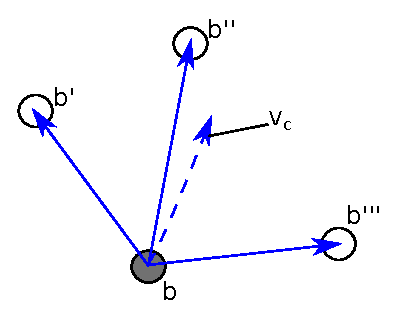
\includegraphics[width=7cm]{CHAPTER-2/figures/FlyToCentre1}
\end{center}
\caption{Cohesion: Origin $b$ \label{methods:FlyToCentre1}}
\end{figure}

The cohesion vector $v_{c}(b)$ for agent $b$ is the resultant vector calculated by summing the vectors $bb'$ formed from the agent to each of its neighbours~$b' \in nbr(b)$~\cite{HAY:08}.

$S$ is the set of all agents that make up the swarm.

\begin{equation}\label{eq:Swarm1}
S \buildrel \Delta \over = \{b'\ldots b^{n}\}
\end{equation}‎

\begin{equation}\label{eq:Neighbours1}
nbr(b) \buildrel \Delta \over = \{b' \in S | b' \text{ is a neighbour of } b\}
\end{equation}‎

\begin{equation}\label{eq:FlyToCentre1}
v_{c}(b) = \frac{\mathlarger{\sum_{b' \in nbr(b)}}{bb'}}{|nbr(b)|}
\end{equation}‎

\section{Swarm repulsion}\label{sec:Repulsion1}
Repulsion is defined by Reynolds, Kawabayashi and Chen, and Shinichi et al. as an agent in a swarm having a fixed distance/range where another agent will be repelled if it moves within that range~\cite{REY:87, KC:08, AYSH:08}. This creates a `field effect' around the agent such that when another agent enters that area a vector is applied to its directional bias to prevent the agents colliding. Repulsion is also applied to agents when they interact with obstacles, this is covered in~\autoref{section:ObstacleSection}.

The repulsive vector is applied at a boundary and the vector is fixed in magnitude~\cite{KC:08, REY:87, AYSH:08}~(\autoref{methods:Repulsion3}). 

\begin{figure}[H]
\begin{center}
\includegraphics[width=7cm]{CHAPTER-2/figures/Repulsion3}
\caption{Agent fixed magnitude repulsion\label{methods:Repulsion3}}
\end{center}
\end{figure}

\subsection{Swarm repulsion application}\label{sec:Repulsion1}
In this thesis a proportional vector will be applied to create a graduated repulsion effect. This is similar to the approach used for the application of cohesion. 

Each neighbouring agent's repulsive effect is applied proportionaly~(\autoref{methods:Repulsion1}). When an agent encroaches upon another agent the degree of the field intrusion is taken into account. This affects the magnitude of the repulsive vectors that are applied~(\autoref{methods:Repulsion4}) and therefore the resultant repulsion vector. 

This technique improves the calculated directional bias such that the calculated direction reduces the probability of a collision. In this thesis the inter-agent repulsion will be calculated as the average of all the proportional repulsion vectors~(\autoref{methods:Repulsion4}). 

\begin{figure}[H]
\begin{center}
\includegraphics[width=8cm]{CHAPTER-2/figures/Repulsion1}
\caption{Proportional agent repulsion \label{methods:Repulsion1}}
\end{center}
\end{figure}
 
\begin{figure}[H]
\begin{center}
\includegraphics[width=7.5cm]{CHAPTER-2/figures/Repulsion2}
\caption{Proportional agent repulsion \label{methods:Repulsion2}}
\end{center}
\end{figure}

Due to the proportional application of the repulsion vector when multiple agents interact the calculated trajectory will not be the mid-point on the intersecting angle but will be offset based upon a positional effect~(\autoref{methods:Repulsion4}). In the case shown in~\autoref{methods:Repulsion4} the positional effect (green) increases the distance agent ($b$) will move away from $b'$. This creates a greater distance than would occur if using a fixed magnitude (blue) vector method. This reduces the chance of a collision between the two agents. The proposed model is therefore more directionally appropriate. 

\begin{figure}[H]
\begin{center}
\includegraphics[width=8cm]{CHAPTER-2/figures/Repulsion4}
\caption{Repulsion comparison\label{methods:Repulsion4}}
\end{center}
\end{figure}

To calculate the total inter-agent repulsion the neighbours that are within the repulsion field must be identified as shown in~\autoref{eq:Repulsion2}.

$R(b)$ is the set of all agents neighbouring $b$ that are repelling $b$. Where $m_b$ is the minimum range for $b$ and $|\overrightarrow{bb'}|$ is the distance between~$b$ and its neighbour~$b'$.  

\begin{equation}
\label{eq:Repulsion2}
R(b) = \{nbr(b):|\overrightarrow{bb'}| < m_b\}
\end{equation}

\autoref{eq:Repulsion1} calculates the final repulsion vector to use for agent $b$ where $v_{r}(b)$ is a repulsive vector generated when neighbouring agents are within the repulsion field effect range. 
When agents move into this area the agent $b$ is repelled in proportion to the amount the neighbours have moved into the agent's repulsion field effect area. The proportion of field intrusion is calculated by $\frac{d_b - |\overrightarrow{bb'}|}{d_b}$. The field effect distance is $m_b$, this is the range around the agent where the repulsion effect is introduced to prevent a collision. 

\begin{equation}
\label{eq:Repulsion1}
v_{r}(b) =‎ -
\frac{1}{|R(b)|}
\left(
\mathlarger{\mathlarger{\sum_{b' \in R(b)}}}
{\left( 1-\frac{|bb'|}{m_b} \right)}
{bb'}
\right)
\end{equation}‎

\section{Swarm model}
The rules of `keep a minimum distance' (repulsion) and `maintain proximity' (cohesion) cause the swarm to form natural geometric structures. These structures tend towards equilateral triangles and when the distribution of the agents allows hexagons are formed. These structures only occur when the repulsive and cohesive fields are set such that the swarm is able to form~\cite{PCL:08, PCL:08a}. The field effects must also be such that the visibility of neighbours does not extend beyond the immediate neighbours of an agent. The effects of field ranges and swarm distribution are covered in more detail in~\autoref{chapter:SwarmType}.  

When cohesion and repulsion vectors are the only vectors acting upon a set of agents and the agents are in close enough proximity to each other, they coalesce into their most stable state. The most stable state is all agents equidistant apart with equal angles. If two agents are in close proximity they will naturally adhere to each other due to the proximity rule~(\autoref{fig:StableForms}). In the case of 3 agents a triangle will form. In the case of 4 agents the most stable shape will be a diamond with the centre agents joined. With 5 and 6 agents a triangular lattice will emerge and with 7 agents a stable hexagon will form. The hexagon~(\autoref{fig:StableFormHexagon}) is the most stable structure with all agents being equidistant and all angles between each neighbouring agent equal~\cite{BAF:06, GP:05}. These structures are seen throughout the natural world~\cite{RAZ:13} and are known to be some of the most stable structures.

\begin{figure}[H]
\begin{center}
\includegraphics[width=7cm]{CHAPTER-2/figures/StableForms}
\end{center}
\caption{Stable swarm formations}\label{fig:StableForms}
\end{figure}

\begin{figure}[H]
\begin{center}
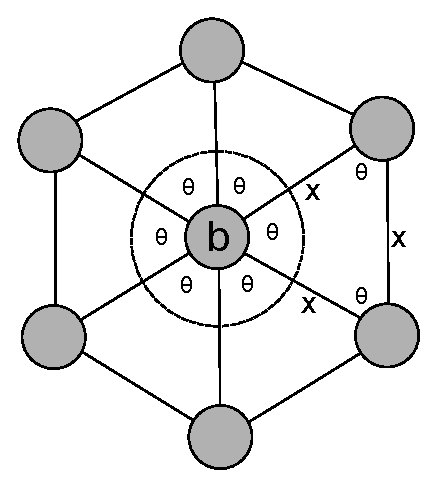
\includegraphics[width=4cm]{CHAPTER-2/figures/Hexagon}
\end{center}
\caption{Stable hexagonal formation}\label{fig:StableFormHexagon}
\end{figure}

\section{Swarm direction}\label{sec:Direction1}
Each agent within a swarm will calculate the repulsion and cohesion vectors based on all their interactions and from those interactions a single vector will be generated by summing the cohesion and repulsion vectors. This resultant vector is then used to determine the agents next position. The position is determined by using the speed characteristic of the agent with the resultant vector. The resultant vector is normalised to produce a directional vector~(\autoref{eq:BotSwarm1}). The directional vector is then used to calculate the agents next position by using the speed characteristic of the agent~\autoref{eq:BotSwarm2} along with the time cycle $t$ of the system~(\autoref{eq:BotSwarm2}). Each agent carries out this process independently and the result is its next position.

The directional vector $v(b)$ for agent $b$ (\autoref{methods:Repulsion1}) is therefore the normalised sum of the cohesion and repulsion vectors.

\begin{center}
\begin{equation}
\label{eq:BotSwarm1}
v(b) =‎ \Big(v_{c}(b) + v_{r}(b)\Big)\string^
\end{equation}‎
\end{center}

Note: \string^ is the equivalent of $\hat{v} = \frac{v}{|v|}$ the normalised vector.

The next location of agent $b$ is $l(b)$ where $s_b$ is the speed of agent~$b$ and $t$ is the time cycle for the movement.

\begin{center}
\begin{equation}
\label{eq:BotSwarm2}
l(b) =‎ \frac{s_{b}}{t}v
\end{equation}‎
\end{center}

\section{Goal based swarm direction}\label{sec:Direction1}
There are two directional aspects to swarm motion. First the motion created by inter-agent reactions through the cohesive and repulsive fields as discussed in~\autoref{sec:Repulsion1} and~\autoref{sec:Cohesion1}. Second is a directional bias applied to a swarm to influence the motion of a swarm in a particular direction. This technique is used in most goal based swarms as discussed by Barnes et al., Bennet and McInnes, Cai et al., Correll and Rus, Dinolov et al. and Ekanayake et al.~\cite{BAF:06, BAFVM:06, BM:09, CML:ND, CR:13, DLK:11, EP:10}. The direction is usually applied at the agent level as a single destination. This thesis will use a single destination for goal based swarms and multiple destinations will be discussed in \autoref{sec:DirectionalShape3} and \autoref{sec:DirectionalShape4}. 

A destination is considered to be a point within a Euclidean plane for a swarm to migrate towards. The directional vector is created by the using the vector generated from the agent to the `point'. This directional vector is normalised and then added to the agent's cohesion and repulsion vectors to create a single `next movement' vector~\cite{BHK:07}. The direction vector is applied as a weighted normalised vector~\autoref{methods:weightedModel}. 

\autoref{eq:Destination1}~calculates the initial vector selection from a group of destinations based on minimum magnitude.

\begin{figure}[H]
\begin{center}
\includegraphics[width=7cm]{CHAPTER-2/figures/Destination1}
\caption{Destination attraction\label{methods:Destination1}}
\end{center}
\end{figure}

\begin{center}
\begin{equation}\label{eq:Destination1}‎
v_{d}(b) =‎ \{bd' | d' \in D | min(b,D)\}
\end{equation}‎
\end{center}

$v_d(b)$ is the resultant destination vector where $D$ is the set of all possible destinations. $b$ is the agent's current position and $d'$ is the nearest destination. $min(b,D)$ returns the destination which has the smallest magnitude in relation to the agent $b$.

\section{Agent resultant direction calculation}
An agent's direction is the sum of all the normalised component vectors~\cite{HAY:08}. For a vector to be used for movement it must have a magnitude of 1 before the agent speed can be applied as shown in~(\autoref{eq:BotDirection1}).

\begin{center}
\begin{equation}
\label{eq:BotDirection1}
v(b) =‎ \Big(v_{c}(b) + v_{r}(b) + v_{d}(b)\Big)\string^
\end{equation}‎
\end{center}

\section{Weighted sum aggregation model}\label{methods:weightedModel}
The purpose of a weighted aggregation model is to alter the level of influence each component of an equation has upon a result. This technique is generally referred to as a `weighted sum aggregation' or `ordered weighted averaging'. This technique is applied to optimisation algorithms such as PSO (Particle Swarm Optimisation) and  involves applying all the possible combinations of the weightings to a multi-variable environment to determine the optimum output~\cite{MV:12, XTH:09}.

\autoref{eq:BotDirection1} is limited in that all the directional vectors are statically applied with the same level of influence.

In this thesis the technique of weighted sum aggregation is applied to the vector calculations to allow tuning of the swarming algorithm of an agent and to change the degree of influence each component has. 

The tuning is implemented as weighting to each component via a weighing factor $k$~\autoref{eq:BotPhysics1}. The weightings ($k_c, k_r, k_d$) are applied before the resultant directional vector is normalised. This change of bias allows levels of importance to be added to a feature i.e. $k_c > k_d$ implies it is more important for the agents to remain connected than it is for them to travel towards the destination. This technique is identified by Muniganti and Pujol in their survey of mathematical modelling techniques as an approach to tailoring a swarms dynamics~\cite{MP:10}. 

Aggregation model weightings can be applied in different ways. The weighting can be applied as a set of arbitrary integer values (12, 67, 99) or as a set of values that always have a summed value of 1 e.g. 0.5, 0.25, 0.25. Either of these techniques are acceptable as the resultant vector is normalised following the weighting application. This thesis implements the weightings as a set of arbitrary integer values~(\autoref{eq:BotPhysics1}). Where $k_c$ is the weighting factor for cohesion, $k_r$ is the weighting factor for repulsion, and $k_d$ is the weighting factor for the destination. 

\begin{equation}\label{eq:BotPhysics1}‎
v(b) =‎ \Big(k_cv_c(b) + k_rv_r(b) + k_dv_d(b)\Big)\string^
\end{equation}‎

\section{Resultant agent model}
The swarm model created in~\autoref{eq:BotPhysics1} with suitable weightings will allow a swarm to form `stable' structures such that the agents will remain connected~(\autoref{methods:Stable1}) and over time migrate to an optimum overall structure for the models parameters. The parameters are the field effect ranges, the cohesion and repulsion magnitude models and the weightings. 

The initial random deployment of a set of agents to create a swarm produces a `chaotic' state. The chaos is caused by the varying cohesion and repulsion vectors that are generated by the inter-agents relationships. Following the initial deployment the magnitudes will create movements that gradually stabalise the swarm structure to a level of movement that best fits the model parameters~\cite{PG:08, WF:12}. The point of equilibrium for the swarm and the resultant structure is dependant upon the agent's cohesion and repulsion fields level of overlapping. This is discussed in section~\autoref{section:AnalysisA} and~\autoref{section:AnalysisB}.

When modelling swarms it is common practice to have the agents in constant motion~\cite{LCW:07, GKF:13}. In this thesis agents are modelled moving at a constant speed with no inertial effect such that an agent can move freely within a Euclidean space. The only exception to this will be if an equilibrium state is encountered. This is where the summed vectors produce a null vector. If this occurs the agent will stop moving.

\section{Repulsion calculation (Obstacles)\label{section:ObstacleSection}}
The model above can be extended to accommodate other enviromental assets by applying additional weighted vectors to~\autoref{eq:BotPhysics1}. Obstacles, like agents, can be represented as a point in the Euclidean plane~(\autoref{section:ObstacleSection}). Obstacles have only one field effect that are modelled as a repulsive effect when an agent moves within an obstacle's field effect.

In this thesis obstacles are modelled with a fixed distance/range where a repulsion vector is applied $d_o$. The repulsion effect is a fixed magnitude of $d_o$. If an agent is within the field effect of more than one obstacle the repulsion vector is the sum of the approach vectors that the agent makes with each of the obstacles~\autoref{eq:Obstacle2} that is normalised and scaled such that the magnitude is the same as the field distance~$d_o$~\autoref{eq:Obstacle2}.

\begin{figure}[H]
\begin{center}
\includegraphics[width=6cm]{CHAPTER-2/figures/Obstacle1}
\end{center}
\caption{Obstacle repulsion \label{methods:Obstacle1}}
\end{figure}

\autoref{eq:Obstacle1} is the set of all agents in the system~$O$ .

\begin{center} \label{eq:Obstacle1}
\begin{equation}‎
O \buildrel \Delta \over =‎ \{o'\ldots o^{n}\}
\end{equation}‎
\end{center}

\autoref{eq:Obstacle4} produces $R(b)$ which is the set of all obstacles that an agent has encroached upon. The obstacles are identified by taking the distance between an agent $|bo'|$ and the fixed field effect for an obstacle~$d_{o}$ and comparing.

\begin{center} \label{eq:Obstacle4}
\begin{equation}‎
R(b) \buildrel \Delta \over =‎ \{o' \in O:|bo'| < d_{o}\}
\end{equation}‎
\end{center}

\autoref{eq:Obstacle2} shows the resultant repulsion vector $v_o(b)$ for an agent. The result is calculated by summing all the scaled normalised vectors $\widehat{bo'}d_{o}$

\begin{center} \label{eq:Obstacle2}
\begin{equation}‎
v_o(b) =‎ \mathlarger{\mathlarger{\mathlarger{\sum}}}_{o' \in R(b)}\widehat{bo'}d_o
\end{equation}‎
\end{center}

%% \begin{center} \label{eq:Obstacle3}
%% \begin{equation}‎
%% v_o(b) =‎ |l_o(b)|d_o
%% \end{equation}‎
%% \end{center}

\subsection{Resultant agent model including obstacle avoidance}\label{methods:AgentModelObstacle}
The initial effect of the swarming algorithms using cohesion, repulsion and direction create a stable mobile swarm~(\autoref{methods:Stable1}). The stability due due to the agents approaching an equilibrium position where all resultant magnitudes balance. 

The addition of the obstacle repulsion~(\autoref{eq:BotPhysics2}) allows the swarm to avoid obstacles that are in its path as it migrates towards its destination. The obstacle avoidance component is weighted~$k_{o}$ to allow the effect to be balanced with the other swarming vectors.

\begin{equation}\label{eq:BotPhysics2}‎
v(b) =‎ \Big(k_cv_c(b) + k_rv_r(b) + k_dv_d(b) + k_ov_o(b)\Big)\string^
\end{equation}‎

\section{Swarm deployment}
Using the methods discussed in this chapter a swarming behaviour emerges from a collection of agents. The initial deployment of a swarm may be a random dispersal of the agents such that the swarm is in a chaotic state~(\autoref{methods:Chaos1}), this chaos is caused by a instability in the magnitudes that are acting upon each of the agents (as detailed above). Based upon the application of the models discussed the swarm will initially move in such a way as to balance all the vectors resulting in a period of organisational chaos in that the swarms goal of traversing an environment will be limited as the vectors generated to disperse the agents will inhibit the directional bias. 

This phase of the swarms life cycle is the `initialisation phase'~(\autoref{methods:StableTime1}). When the initialisation phase is over the vector calculations (cohesion, repulsion, and direction) will balance and the swarm will create stable shapes such as hexagonal lattices where all the angles and lengths (distances between agents) tend toward being equal~(\autoref{methods:Stable1})

Theses effects can be seem in the screenshots (Figures \ref{methods:Chaos1}, \ref{methods:Chaos1}, \ref{methods:Stable1}) from the simulator discussed in \autoref{chapter:simulator}.

\begin{figure}[H]
\begin{center}
\includegraphics[width=7cm]{CHAPTER-2/figures/Chaos}
\end{center}
\caption{Chaotic swarm\label{methods:Chaos1}}
\end{figure}

\begin{figure}[H]
\begin{center}
\includegraphics[width=7cm]{CHAPTER-2/figures/Stable}
\end{center}
\caption{Stable swarm\label{methods:Stable1}}
\end{figure}

\begin{figure}[H]
\begin{center}
\includegraphics[width=10cm]{CHAPTER-2/figures/StableTime}
\end{center}
\caption{Swarm stabalisation\label{methods:StableTime1}}
\end{figure}

\section{Conclusion}
This chapter discusses the mathematical modelling of swarms used throughout this thesis. The modelling covers the cohesion model to ensure agents remain part of a cohesive body and the repulsive model used to ensure agents do not collide and thefore maintain a stable swarming structure. The chapter also introduces two additional aspects of swarming to the model; directional bias and obstacle avoidance. These are all combined to create the model required for this thesis. 


